\chapter{Descripción del proyecto}
En este capítulo se describe cómo funciona el motor en esencia, es decir, sin entrar en la implementación del mismo. Esta idea general no depende del lenguaje de programación.

Hay un apartado que describe al motor y sus capacidades, y otro apartado que muestra el diseño actual de la aplicación y expone otras ideas que se pueden llevar a cabo.

\section{Qué es un motor de videojuegos (Descripción)}

El programa que se ha desarrollado es un motor que funciona como \textbf{intérprete de videojuegos}. Permite a un usuario cualquiera reproducir un videojuego definido en un formato predefinido. Este formato permite abstraer de toda la capa programática a un diseñador.

Aunque lo parezca, y quizás en una futura compilación sea capaz de hacerlo, no es una aplicación que permita crear un videojuego, sino que es capaz de reproducir videojuegos creados por un usuario.

El proyecto también se le puede definir como un motor de videojuegos:
\begin{quote}
	\small Un motor de videojuego es un término que hace referencia a una serie de librerías de programación que permiten el diseño, la creación y la representación de un videojuego. \cite{Alberto_Carrasco}
\end{quote}

En este caso, el proyecto no es una serie de librerías sino que es directamente una aplicación. De esta manera, se puede abstraer a un creador del videojuego de la programación directa de un juego.

\subsection{Qué tipo de videojuegos se pueden crear}
El interprete está orientado a reproducir juegos en los que el jugador tiene que escapar de una mazmorra. Para ello, el jugador debe reunir objetos como llaves para abrir puertas, esquivar trampas, resolver rompecabezas, luchar contra monstruos, usar pociones y llegar a una habitación final.
Algunos ejemplos de juegos parecidos a los que está orientado el motor son ''Dragones y Mazmorras'' o los libros de ''elige tu propia aventura''.

Aunque el motor esté desarrollado con una fuerte influencia por este tipo de juegos, no está limitado a ellos, cualquier creador pueda ir más allá de este concepto o incluso cambiarlo radicalmente usando las herramientas genéricas de las que dispone el motor. El límite lo pone la imaginación del usuario.

\subsection{Dónde se podrá usar el motor}
De momento sólo está disponible para dispositivos que soporten el sistema operativo iOS, es decir, solo para dispositivos portables de Apple, como un iPhone o un iPad.
Tampoco hay planes actuales de mover el motor a otra plataforma, pero es posible implementar el motor en otros sistemas y lenguajes de programación.

Con todas estas dudas resueltas ya solo queda mostrar las funciones de las que dispone el motor.

\subsection{Qué es capaz de hacer el motor}

El proyecto anterior se considera un punto de partida para muchos conceptos que se querían llevar a cabo para el nuevo motor. Por ello, se escogieron ciertas funcionalidades comunes que permitieran representar al videojuego original, separandolas en pequeñas piezas: mostrar un diálogo, iniciar un combate...
De esta manera nacen los eventos.

\subsection{Eventos}

Un \textbf{evento} representa una acción atómica que puede realizar el motor. Estas acciones se consideran básicas en el ámbito de una aventura, como escoger una opción o mostrar un diálogo; aunque requieran de más trabajo a la hora de programarlas.

Los eventos están pensados para unirse entre ellos, de manera que se puedan mezclar entre sí varias acciones básicas para formar una cadena de eventos. Por ello, cualquiera de ellos son intercambiables, intercalables y no pueden tener dependencias entre sí.
Además, siempre se ejecutan de forma lineal, siguiendo un orden predefinido por el creador del juego.

El centro de toda la potencia del motor reside en los eventos, ya que son un mecanismo genérico y preciso de ejecutar acciones en el juego. El motor está encargado de leer cada uno de estos eventos y ejecutar una acción según el contenido del mismo.
Otra funcionalidad clave del motor es que nunca sabe el estado en el que se encuentra la cadena de eventos, se conforma con guardar el evento que esté ejecutando en el momento, ejecutarlo y pasar al siguiente.

\begin{figure}[h]
	\caption{Cadena de eventos}
	\centering
	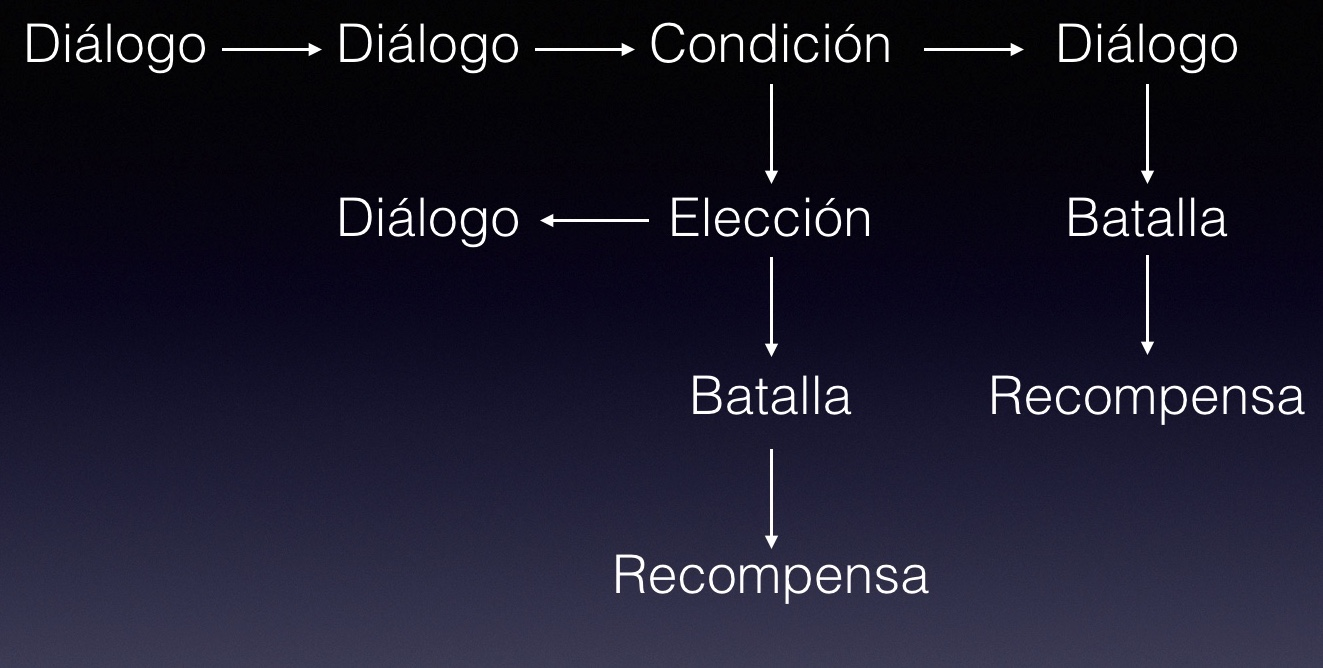
\includegraphics[width=0.75\textwidth]{include/eventsChainExample.jpg}
	
	La idea detrás de los eventos es muy sencilla: al interactuar el usuario con una parte de la aplicación activa una cadena. El evento principal tiene una referencia a otro evento, al que le da paso cuando termina el original. Este encadenamiento sigue hasta que uno de los eventos no tenga ninguna referencia a un evento siguiente, permitiendo que la cadena termine.
\end{figure}

Ahora vamos a definir los tipos de eventos que existen, las acciones que conllevan dentro del motor y sus posibles usos. Respecto a diseño que toman, se describirá más adelante en la sección de diseño \ref{designSection}. 

\subsubsection{Diálogo}
Evento que muestra un mensaje dicho por un personaje en el videojuego. La mayor traba del proyecto original era que los diálogos correspondían con la mayor parte del código fuente, por lo que este evento permite quitar mucha lógica duplicada en el código.

Su uso más frecuente es para mostrar conversaciones entre personajes, aunque también se puede usar para escribir los pensamientos del protagonista, describir una sala o un personaje, plantear un problema...

\subsubsection{Condición}
Evento que verifica una condición sobre el estado actual del juego. Este evento es transparente para el usuario, ya que se ejecutará un evento u otro siguiente dependiendo de si la condición es cierta o no. Las condiciones son las que se describen en la sección \ref{conditionsSubsection}.

Este evento se suele usar cuando se quiere evaluar el estado del juego y tomar acciones en consecuencia. Por ejemplo, diálogos dependientes del compañero, cofres que no se abren si no dispones de una llave...

\subsubsection{Elección}
Evento que permite al jugador escoger entre una serie de opciones. Dependiendo de la opción escogida, se ejecutará un evento u otro. Además, las opciones pueden incluir una condición para que se muestren, como las descritas en la sección \ref{conditionsSubsection}.

Algunos ejemplos en los que aparece este evento son cuando hay que resolver un acertijo y se muestran varias respuestas, o cuando un personaje te ofrece posibles formas de pago para un trueque.

\subsubsection{Batalla}
Evento que inicia una nueva batalla con la información de un enemigo al que enfrentarse.
Hasta que no termine la batalla no se pasará al siguiente evento de la cadena.

Al terminar la batalla se ejecutará un evento según si el jugador ha ganado o ha perdido.

\subsubsection{Recompensa}
Evento que agrega objetos al inventario del jugador. En ningún caso agregará objetos que no existan en el videojuego.

Se suele usar para recompensar a un jugador por haber ganado una batalla o por haber abierto un cofre.

\subsection{Habitaciones}
La idea original para el desarrollo del juego es un laberinto. Un laberinto se puede representar como una serie de pasillos delgados y oscuros por los que el protagonista debe orientarse, o como una serie de habitaciones interconectadas entre sí.
Esta última opción nos permite obtener mayor detalle sobre los eventos y ayudar al jugador a recordar la estructura del laberinto. 

Una habitación es el sitio donde ocurren todos los eventos que se pueden encontrar en el juego. Es en estos lugares donde el jugador va a tener mayor libertad de movimientos porque es el lugar donde se ejecutan cadenas de eventos, puede ir hacia otras habitaciones o donde puede guardar la partida y cambiar ciertos ajustes.

Está representada con una imagen principal que describe a la habitación junto con un título y una descripción, y una serie de acciones que puede realizar el jugador dentro de ella.

\subsection{Personajes}
Durante la aventura el protagonista puede interactuar con múltiples personajes: compañeros, enemigos y NPCs, las siglas de \textit{''non playable character''}. \cite{npcGeekno} Además, el jugador también cuenta como un personaje aparte.

Los personajes contienen un nombre y una imagen que los representa, aparte de una serie de características como la resistencia que tiene en batalla y otras estadísticas.

Los personajes por lo tanto son piezas esenciales de la acción durante el juego por distintas razones:

\begin{itemize}
	\item Los diálogos siempre son enunciados por alguien, que debe ser un personaje.
	\item El protagonista y su compañero tienen una serie de características que son cruciales para la evaluación de condiciones.
	\item En una batalla, siempre luchan un personaje enemigo con el protagonista y sus compañeros.
\end{itemize}

Además, usar personajes permite que los jugadores puedan adentrarse en la aventura con mayor facilidad e incluso identificarse con ellos.

\subsection{Condiciones} \label{conditionsSubsection}
El motor tiene varios puntos donde se necesita ejecutar condiciones para resolver ciertas acciones. Estas condiciones dependen de varios factores como las estadísticas del protagonista, las variables, etc.

Existen varios tipos de evaluaciones:
\begin{itemize}
	\item Compañero: si el protagonista tiene un compañero que coincide con el nombre definido, entonces la condición se evalúa a verdadera. En otro caso, la condición es falsa.
	\item Objeto: si el protagonista tiene un objeto en su inventario que coincide con el objeto del evento, entonces la condición es cierta. En otro caso, no se cumple la condición. Es importante puntualizar que si la condición es cierta, entonces el objeto del inventario desaparece o se consume.
	\item Estado de habitación: dependiendo si el protagonista ha visitado una habitación específica o no, la condición se evalúa a cierto o falso. Hay una condición que sirve para saber si se ha visitado una habitación y otra para si no la ha visitado.
	\item Relación de variables: si la relación entre dos variables se cumple, entonces la condición es cierta. En otro caso, la condición es falsa. La relación de variables se describe mejor en la sección \ref{variablesSection}.
\end{itemize}

\subsection{Variables personalizadas} \label{variablesSection}

\section{Qué esperar del sistema (Diseño)} \label{designSection}

\section{Cómo se ve el motor en funcionamiento}

\section{Guía para usar el sistema}

Antes de comenzar, todos los eventos tienen una serie de características comunes entre ellos:

\begin{itemize}
	\item Identificador: todos los eventos cuentan con un id, y este debe ser único. No se asegura que dos eventos con identificadores idénticos funcionen a la vez.
	\item Siguiente paso: indica el identificador del próximo evento a ejecutarse...
	akbhdfdkjalskshbebbjdkjbajbkRELLENAR
\end{itemize}

Para crear un videojuego disponemos de x archivos.
Describir cada uno y explicar en qué se traduce en el juego

\subsection{Música}

\chapter{Desarrollo de la aplicación}

\section{Una manera de llevarlo a cabo (Arquitectura)}

\section{Desarrollando en dispositivos móviles (Implementación)}